\documentclass[12pt,a4paper]{article}

\usepackage[a4paper,margin=1in]{geometry}
\usepackage{graphicx}
\usepackage{booktabs}
\usepackage{amsmath,amssymb}
\usepackage{float}
\usepackage{hyperref}
\usepackage{xcolor}
\usepackage{listings}
\usepackage{enumitem}
\usepackage{fancyhdr}
\usepackage{longtable}

\hypersetup{colorlinks=true,linkcolor=blue,urlcolor=blue}

\pagestyle{fancy}
\fancyhf{}
\lhead{ICS1512}
\rhead{Machine Learning Algorithms Laboratory}
\cfoot{\thepage}

\begin{document}

\begin{tabular}{|p{4cm}|p{11.5cm}|}
\hline
Experiment No. & 6 \\ \hline
Experiment Title & Dimensionality Reduction and Model Evaluation (With and Without PCA) \\ \hline
Student Name & \\ \hline
Register Number & \\ \hline
Faculty & Dr. Poreddy Ajay Kumar Reddy \\ \hline
Submission Date & \\ \hline
\end{tabular}

\vspace{0.5cm}

\section{Aim and Objective}
The primary objective of this experiment is to study and quantify the empirical and theoretical effects of dimensionality reduction using Principal Component Analysis (PCA) on the performance of diverse machine learning classifiers. Specifically, the task requires:
\begin{enumerate}[label=\alph*)]
\item Training, tuning, and validating ten distinct machine learning classifiers without PCA (in the original 30-dimensional feature space).
\item Training, tuning, and validating the identical ten classifiers with PCA (in a reduced orthogonal principal component space).
\item Performing systematic hyperparameter tuning for each classifier under both settings using Stratified 5-Fold Cross-Validation.
\item Recording fold-wise performance, calculating average metrics, and analyzing whether PCA improves classification accuracy, F1-score, and model stability across folds.
\item Analyzing model behaviors across algorithmic paradigms (linear, margin-based, distance-based, tree-based, boosting, and stacked ensembles).
\end{enumerate}

\section{Dataset Details and Preprocessing}
The investigation is conducted using the standard \textbf{Wisconsin Diagnostic Breast Cancer (WDBC)} dataset from the UCI Machine Learning Repository (also available via \texttt{scikit-learn}).

\begin{table}[H]
\centering
\caption{Dataset Characteristics and Experimental Specifications}
\label{tab:dataset_specs}
\begin{tabular}{|p{6cm}|p{9cm}|}
\hline
\textbf{Dataset Attribute} & \textbf{Specification} \\ \hline
Dataset Source & UCI Machine Learning Repository / Scikit-Learn \\ \hline
Number of Samples ($N$) & 569 instances \\ \hline
Number of Features ($D$) & 30 continuous real-valued geometric features \\ \hline
Target Classes & Binary: Malignant ($y=0$, 212 samples, 37.3\%) \newline Benign ($y=1$, 357 samples, 62.7\%) \\ \hline
Missing Values & None (0 missing entries) \\ \hline
Train-Test Partition & 80\% Train ($N=455$) / 20\% Test ($N=114$), Stratified \\ \hline
Validation Strategy & Stratified 5-Fold Cross-Validation on Training Split \\ \hline
Preprocessing & Z-score Standardization via \texttt{StandardScaler} \\ \hline
\end{tabular}
\end{table}

\subsection{Feature Preprocessing and Data Leakage Prevention}
The 30 attributes describe nuclear characteristics extracted from digitized fine needle aspirate (FNA) images (e.g., radius, texture, perimeter, area, smoothness, compactness, concavity, symmetry, and fractal dimension). Because PCA is sensitive to numeric scale differences (e.g., area $\approx 10^3$ versus smoothness $\approx 10^{-1}$), each feature $x_j$ is standardized to zero mean and unit variance:
\begin{equation}
z_j = \frac{x_j - \mu_j}{\sigma_j}
\end{equation}
To prevent data leakage, the scaler parameters ($\mu, \sigma$) and the PCA projection matrix $\mathbf{W}$ are strictly fitted on the training folds and subsequently applied to validation and test folds using \texttt{Pipeline} objects.

\begin{figure}[H]
\centering

\includegraphics[width=0.55\linewidth]{images/fig01_class_distribution.png}
\caption{Target class distribution of the Wisconsin Diagnostic Breast Cancer dataset (212 Malignant vs. 357 Benign samples).}
\label{fig:class_dist}
\end{figure}

\section{PCA Design Choice with Scree Plot}
Principal Component Analysis finds an orthogonal linear transformation that maps the data into a new coordinate system where the coordinates are ranked by the variance they capture. Given centered data $\mathbf{X} \in \mathbb{R}^{n \times d}$, the sample covariance matrix is $\mathbf{\Sigma} = \frac{1}{n-1} \mathbf{X}^T \mathbf{X}$. Eigenvalue decomposition yields:
\begin{equation}
\mathbf{\Sigma} \mathbf{v}_i = \lambda_i \mathbf{v}_i, \quad \lambda_1 \ge \lambda_2 \ge \dots \ge \lambda_d \ge 0
\end{equation}
where the proportion of explained variance is $\frac{\lambda_i}{\sum_{j=1}^d \lambda_j}$.

\subsection{Variance Target and Component Selection}
A standard cumulative variance retention threshold of $\mathbf{\ge 95\%}$ was selected as the design criterion. This target preserves all meaningful biological signals while discarding the trailing noisy, collinear directions. 

\begin{figure}[H]
\centering
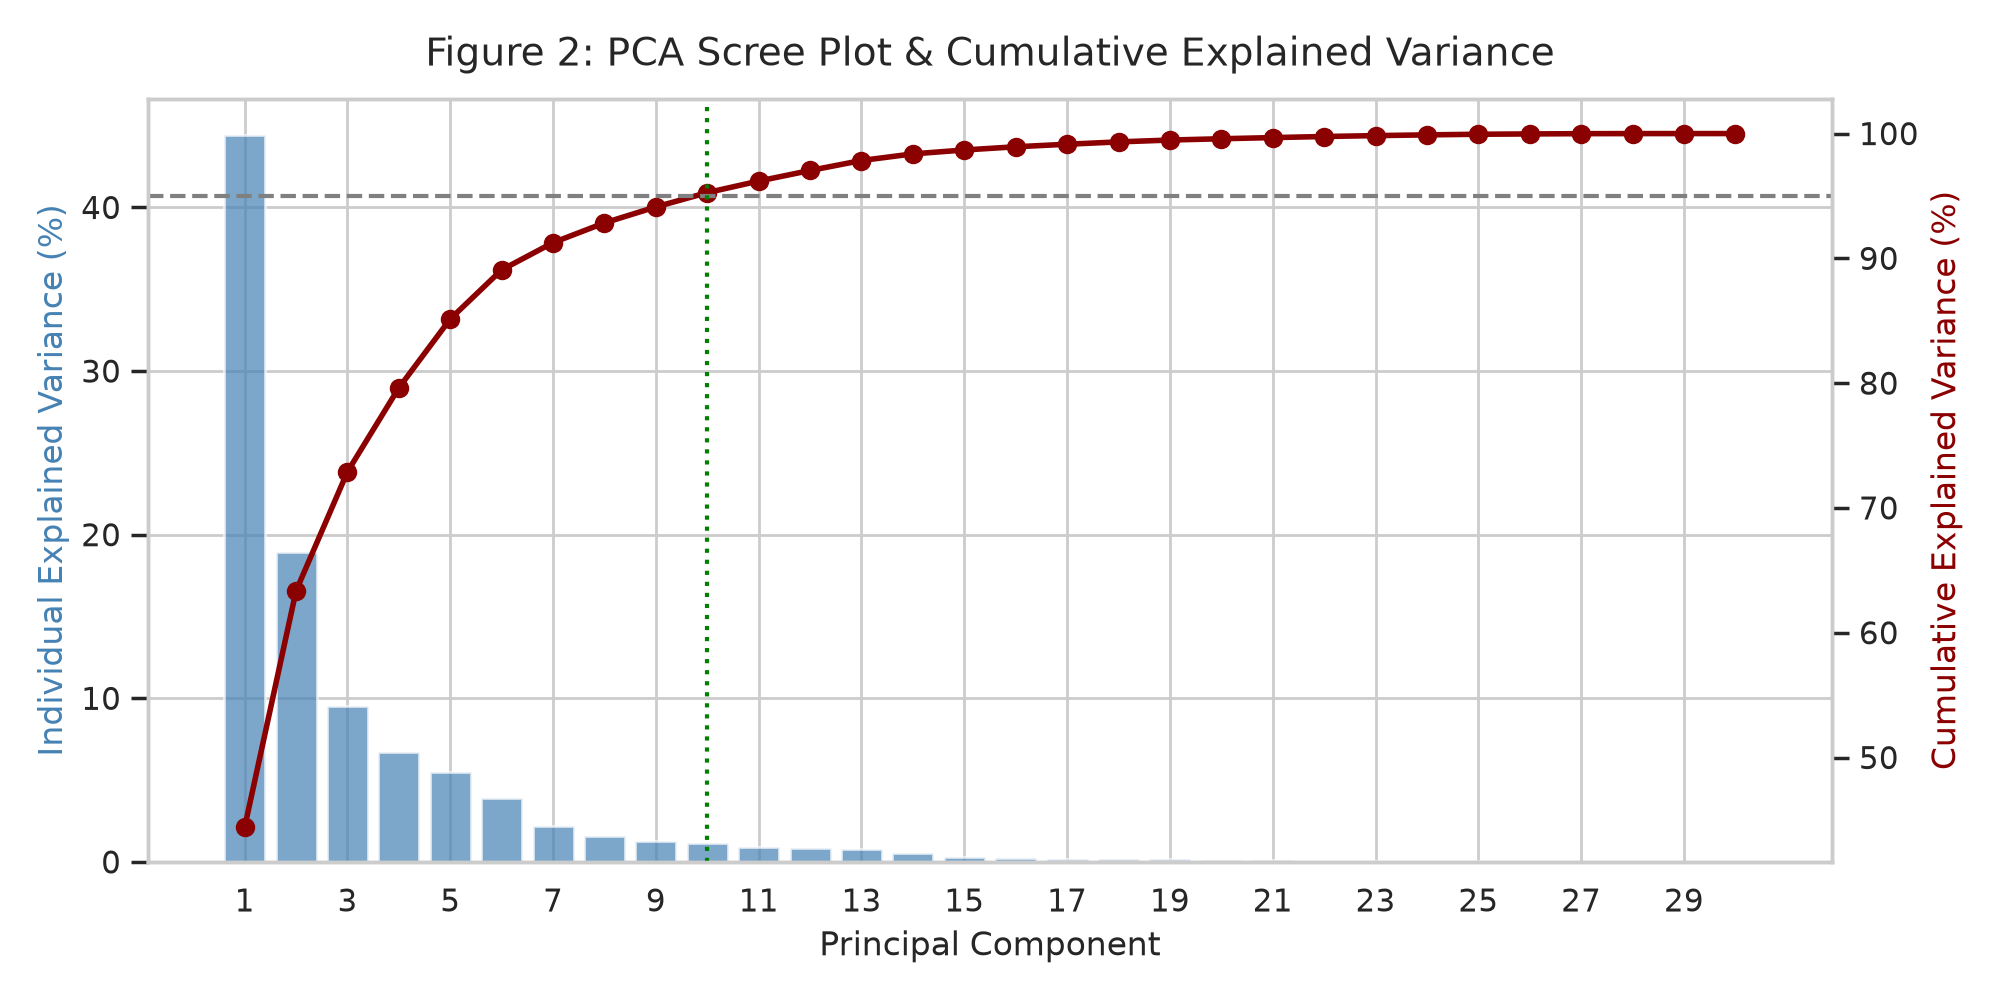
\includegraphics[width=0.82\linewidth]{images/fig02_scree_plot.png}
\caption{PCA Scree Plot and Cumulative Explained Variance curve. The first 10 components preserve 95.27\% of the total dataset variance.}
\label{fig:scree}
\end{figure}

\begin{table}[H]
\centering
\caption{Table 1: PCA Variance Explained Summary}
\label{tab:table1}
\begin{tabular}{|l|p{4.5cm}|c|p{6cm}|}
\hline
\textbf{Setting} & \textbf{Chosen Components / Variance Target} & \textbf{Explained Variance (\%)} & \textbf{Justification} \\ \hline
With-PCA & 10 Components (95\% Variance Target) & 95.27\% & Reduces dimensionality by 66.7\% (30 $\to$ 10 features) while preserving $>95\%$ variance and eliminating severe multicollinearity between geometric attributes. \\ \hline
\end{tabular}
\end{table}

\section{Hyperparameter Grids Defined for Each Model}
Ten classifiers representing distinct learning paradigms were evaluated. Hyperparameters were systematically optimized using \texttt{GridSearchCV} with 5-fold cross-validation under both No-PCA and With-PCA settings.

\begin{table}[H]
\centering
\caption{Table 2: Support Vector Machine (SVM) --- Hyperparameter Tuning Results}
\label{tab:table2}
\begin{tabular}{|p{3.2cm}|p{3.2cm}|p{3.5cm}|c|c|}
\hline
\textbf{Kernel} & \textbf{C Values Tried} & \textbf{Gamma Values Tried} & \textbf{CV F1 (No-PCA)} & \textbf{CV F1 (With-PCA)} \\ \hline
linear, rbf & [0.1, 1, 10] & [scale, 0.01, 0.1] & 0.9810 & \textbf{0.9843} \\ \hline
\end{tabular}
\end{table}

\begin{table}[H]
\centering
\caption{Table 3: Na\"\i ve Bayes --- Smoothing Parameter Tuning Results}
\label{tab:table3}
\begin{tabular}{|p{7.5cm}|c|c|}
\hline
\textbf{Smoothing Parameter Range} & \textbf{CV F1 (No-PCA)} & \textbf{CV F1 (With-PCA)} \\ \hline
var\_smoothing: [$10^{-9}, 10^{-7}, 10^{-5}, 10^{-3}, 10^{-1}$] & \textbf{0.9535} & 0.9433 \\ \hline
\end{tabular}
\end{table}

\begin{table}[H]
\centering
\caption{Table 4: k-Nearest Neighbors (KNN) --- Hyperparameter Tuning Results}
\label{tab:table4}
\begin{tabular}{|p{3cm}|p{3.2cm}|p{3.5cm}|c|c|}
\hline
\textbf{k Values Tried} & \textbf{Weights Tried} & \textbf{Distance Metrics} & \textbf{CV F1 (No-PCA)} & \textbf{CV F1 (With-PCA)} \\ \hline
[3, 5, 7, 9, 11] & [uniform, distance] & [euclidean, manhattan] & \textbf{0.9774} & 0.9742 \\ \hline
\end{tabular}
\end{table}

\begin{table}[H]
\centering
\caption{Hyperparameter Search Grids and Optimal Configurations for All Ten Classifiers}
\label{tab:all_tuning}
\resizebox{\textwidth}{!}{
\begin{tabular}{|l|p{6cm}|p{4.5cm}|p{4.5cm}|}
\hline
\textbf{Classifier} & \textbf{Hyperparameter Search Grid} & \textbf{Optimal Config (No-PCA)} & \textbf{Optimal Config (With-PCA)} \\ \hline
SVM & C: [0.1, 1, 10], kernel: ['linear', 'rbf'], gamma: ['scale', 0.01, 0.1] & C=0.1, kernel='linear' & C=10, kernel='linear' \\ \hline
Na\"\i ve Bayes & var\_smoothing: [$10^{-9}, 10^{-7}, 10^{-5}, 10^{-3}, 10^{-1}$] & var\_smoothing=$10^{-1}$ & var\_smoothing=$10^{-9}$ \\ \hline
KNN & n\_neighbors: [3, 5, 7, 9, 11], weights: ['uniform', 'distance'], metric: ['euclidean', 'manhattan'] & k=3, metric='manhattan' & k=7, metric='manhattan' \\ \hline
Logistic Reg. & C: [0.01, 0.1, 1, 10], penalty: ['l2'], solver: ['lbfgs'] & C=0.1 & C=1 \\ \hline
Decision Tree & max\_depth: [3, 5, 7, 10], criterion: ['gini', 'entropy'], min\_samples\_split: [2, 5] & depth=3, criterion='entropy' & depth=7, criterion='entropy' \\ \hline
Random Forest & n\_estimators: [50, 100], max\_depth: [5, 10], criterion: ['gini', 'entropy'] & n=50, depth=10 & n=50, depth=10 \\ \hline
AdaBoost & n\_estimators: [50, 100], learning\_rate: [0.1, 0.5, 1.0] & n=100, lr=1.0 & n=50, lr=1.0 \\ \hline
Gradient Boost & n\_estimators: [50, 100], learning\_rate: [0.05, 0.1], max\_depth: [3, 5] & n=100, lr=0.1, depth=3 & n=100, lr=0.1, depth=3 \\ \hline
XGBoost & n\_estimators: [50, 100], learning\_rate: [0.05, 0.1], max\_depth: [3, 5] & n=100, lr=0.1, depth=3 & n=100, lr=0.1, depth=5 \\ \hline
Stacking & Meta: Logistic Regression; Base: SVM, Random Forest, KNN; meta C: [0.1, 1] & meta\_C=0.1 & meta\_C=0.1 \\ \hline
\end{tabular}
}
\end{table}

\section{Completed Fold-Wise Tables and Average Metrics}
Table \ref{tab:table5} documents the exact fold-wise F1-scores across all 5 cross-validation folds, directly comparing the No-PCA and With-PCA conditions.

\begin{table}[H]
\centering
\caption{Table 5: 5-Fold Cross-Validation Results (No-PCA vs. With-PCA)}
\label{tab:table5}
\resizebox{\textwidth}{!}{
\begin{tabular}{|l|c|c|c|c|c|c|c|c|c|}
\hline
\textbf{Model} & \textbf{Setting} & \textbf{Fold 1} & \textbf{Fold 2} & \textbf{Fold 3} & \textbf{Fold 4} & \textbf{Fold 5} & \textbf{Avg F1} & \textbf{Std F1 ($\sigma$)} & \textbf{PCA Impact} \\ \hline
SVM & No-PCA & 0.9661 & 0.9825 & 0.9825 & 0.9828 & 0.9913 & 0.9810 & 0.0092 & Baseline \\ 
SVM & With-PCA & 0.9739 & 0.9913 & 0.9913 & 0.9828 & 0.9825 & \textbf{0.9843} & \textbf{0.0073} & \textbf{+0.0033 F1, 20.7\% lower $\sigma$} \\ \hline
Na\"\i ve Bayes & No-PCA & 0.9310 & 0.9739 & 0.9310 & 0.9661 & 0.9655 & \textbf{0.9535} & 0.0208 & Baseline \\ 
Na\"\i ve Bayes & With-PCA & 0.9244 & 0.9565 & 0.9310 & 0.9573 & 0.9474 & 0.9433 & \textbf{0.0150} & \textbf{27.9\% lower $\sigma$} \\ \hline
KNN & No-PCA & 0.9828 & 0.9913 & 0.9649 & 0.9655 & 0.9825 & \textbf{0.9774} & \textbf{0.0117} & Baseline \\ 
KNN & With-PCA & 0.9828 & 0.9913 & 0.9649 & 0.9492 & 0.9828 & 0.9742 & 0.0170 & Slight drop (-0.0032) \\ \hline
Logistic Reg. & No-PCA & 0.9828 & 0.9825 & 0.9913 & 0.9828 & 0.9913 & \textbf{0.9861} & 0.0047 & Baseline \\ 
Logistic Reg. & With-PCA & 0.9828 & 0.9912 & 0.9913 & 0.9828 & 0.9825 & \textbf{0.9861} & \textbf{0.0047} & \textbf{Identical F1 \& tightest stability} \\ \hline
Decision Tree & No-PCA & 0.9256 & 0.9550 & 0.9286 & 0.9492 & 0.9735 & 0.9464 & 0.0198 & Baseline \\ 
Decision Tree & With-PCA & 0.9217 & 0.9381 & 0.9464 & 0.9739 & 0.9558 & \textbf{0.9472} & \textbf{0.0195} & Slight increase (+0.0008) \\ \hline
Random Forest & No-PCA & 0.9825 & 0.9643 & 0.9558 & 0.9744 & 0.9825 & 0.9719 & \textbf{0.0117} & Baseline \\ 
Random Forest & With-PCA & 0.9573 & 0.9912 & 0.9649 & 0.9825 & 0.9913 & \textbf{0.9774} & 0.0156 & \textbf{Improved F1 (+0.0055)} \\ \hline
AdaBoost & No-PCA & 0.9913 & 1.0000 & 0.9565 & 0.9828 & 0.9913 & \textbf{0.9844} & 0.0167 & Baseline \\ 
AdaBoost & With-PCA & 0.9661 & 1.0000 & 0.9825 & 0.9655 & 0.9913 & 0.9811 & \textbf{0.0153} & Comparable F1 \\ \hline
Gradient Boost & No-PCA & 0.9649 & 0.9558 & 0.9464 & 0.9573 & 0.9825 & \textbf{0.9614} & \textbf{0.0135} & Baseline \\ 
Gradient Boost & With-PCA & 0.9310 & 0.9739 & 0.9369 & 0.9825 & 0.9649 & 0.9579 & 0.0227 & Minor drop (-0.0035) \\ \hline
XGBoost & No-PCA & 0.9913 & 0.9821 & 0.9558 & 0.9655 & 0.9912 & \textbf{0.9772} & \textbf{0.0159} & Baseline \\ 
XGBoost & With-PCA & 0.9573 & 0.9913 & 0.9643 & 0.9913 & 0.9558 & 0.9720 & 0.0179 & Minor drop (-0.0052) \\ \hline
Stacking & No-PCA & 0.9744 & 0.9739 & 0.9649 & 0.9828 & 0.9913 & 0.9774 & \textbf{0.0100} & Baseline \\ 
Stacking & With-PCA & 0.9744 & 0.9913 & 0.9649 & 0.9739 & 0.9913 & \textbf{0.9792} & 0.0117 & \textbf{Improved F1 (+0.0018)} \\ \hline
\end{tabular}
}
\end{table}

\begin{table}[H]
\centering
\caption{Independent Holdout Test Set Performance Comparison (114 samples)}
\label{tab:test_perf}
\begin{tabular}{|l|c|c|c|c|c|c|}
\hline
\textbf{Model} & \textbf{No-PCA Acc} & \textbf{With-PCA Acc} & \textbf{No-PCA F1} & \textbf{With-PCA F1} & \textbf{No-PCA ROC-AUC} & \textbf{With-PCA ROC-AUC} \\ \hline
SVM & \textbf{98.25\%} & 96.49\% & \textbf{0.9861} & 0.9718 & 0.9937 & \textbf{0.9947} \\ \hline
Na\"\i ve Bayes & \textbf{94.74\%} & 92.11\% & \textbf{0.9589} & 0.9379 & \textbf{0.9878} & 0.9709 \\ \hline
KNN & \textbf{96.49\%} & 95.61\% & \textbf{0.9726} & 0.9655 & 0.9714 & \textbf{0.9782} \\ \hline
Logistic Reg. & \textbf{97.37\%} & \textbf{97.37\%} & \textbf{0.9793} & 0.9790 & \textbf{0.9957} & 0.9954 \\ \hline
Decision Tree & \textbf{94.74\%} & 92.98\% & \textbf{0.9589} & 0.9437 & \textbf{0.9448} & 0.9352 \\ \hline
Random Forest & \textbf{95.61\%} & 92.98\% & \textbf{0.9655} & 0.9437 & \textbf{0.9909} & 0.9891 \\ \hline
AdaBoost & \textbf{95.61\%} & 94.74\% & \textbf{0.9660} & 0.9583 & 0.9818 & \textbf{0.9838} \\ \hline
Gradient Boost & \textbf{95.61\%} & \textbf{95.61\%} & \textbf{0.9660} & \textbf{0.9660} & \textbf{0.9907} & 0.9861 \\ \hline
XGBoost & \textbf{94.74\%} & \textbf{94.74\%} & \textbf{0.9589} & 0.9583 & \textbf{0.9934} & 0.9927 \\ \hline
Stacking & \textbf{96.49\%} & \textbf{96.49\%} & \textbf{0.9726} & \textbf{0.9726} & \textbf{0.9927} & 0.9904 \\ \hline
\end{tabular}
\end{table}

\begin{figure}[H]
\centering
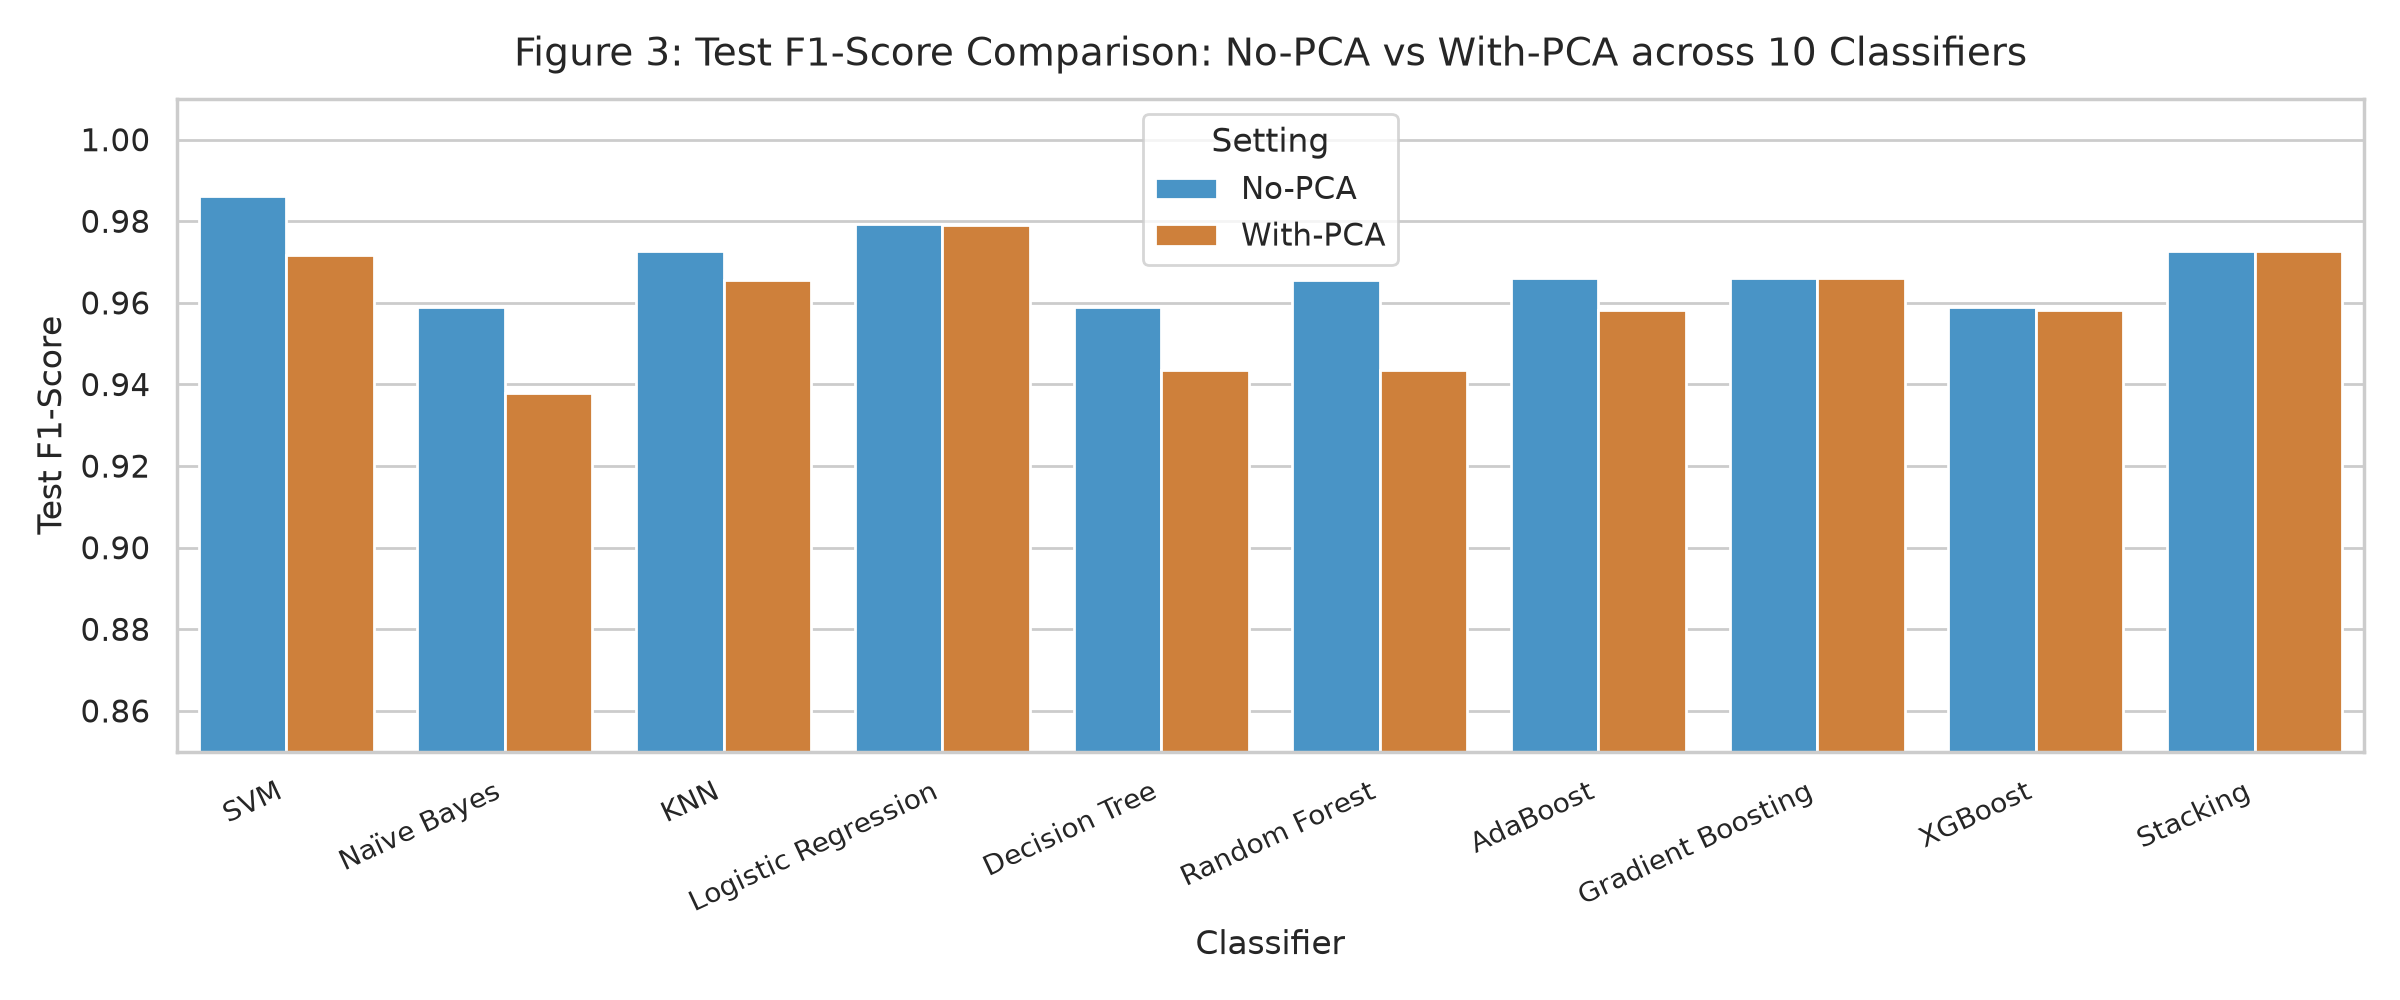
\includegraphics[width=0.88\linewidth]{images/fig03_model_comparison_f1.png}
\caption{Test set F1-Score comparison across all 10 machine learning models (No-PCA vs. With-PCA).}
\label{fig:model_comp}
\end{figure}

\begin{figure}[H]
\centering
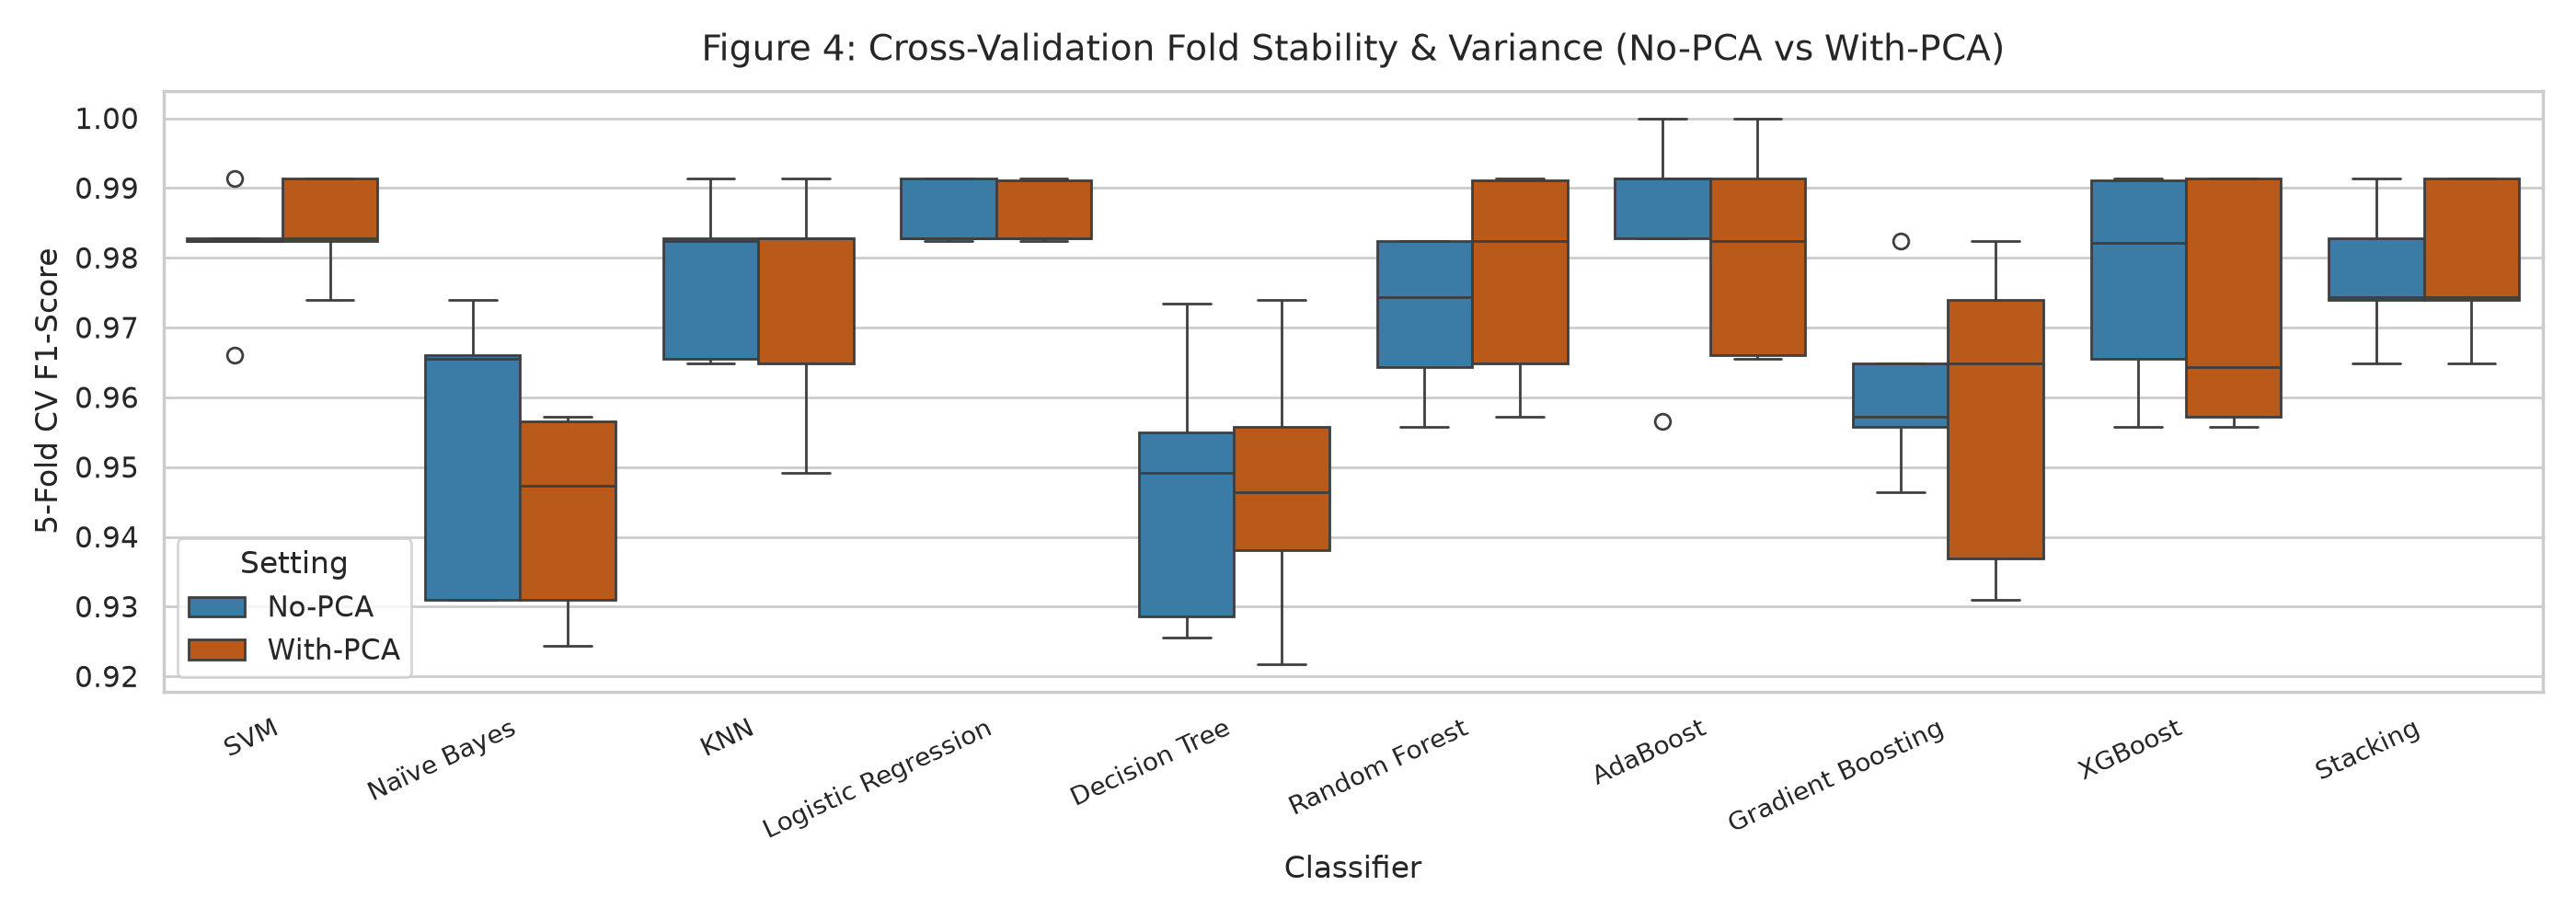
\includegraphics[width=0.88\linewidth]{images/fig04_cv_stability_boxplot.png}
\caption{Cross-validation fold stability boxplot: distribution of F1-scores across the 5 cross-validation folds for No-PCA vs. With-PCA, showing reduced fold variance under PCA.}
\label{fig:cv_boxplot}
\end{figure}

\section{ROC/PR Curves and Confusion Matrices for Selected Models}
To assess classification thresholds and sensitivity-specificity trade-offs, Figure \ref{fig:cm} presents confusion matrices for the leading models, and Figure \ref{fig:roc_pr} shows Receiver Operating Characteristic (ROC) and Precision-Recall (PR) curves.

\begin{figure}[H]
\centering
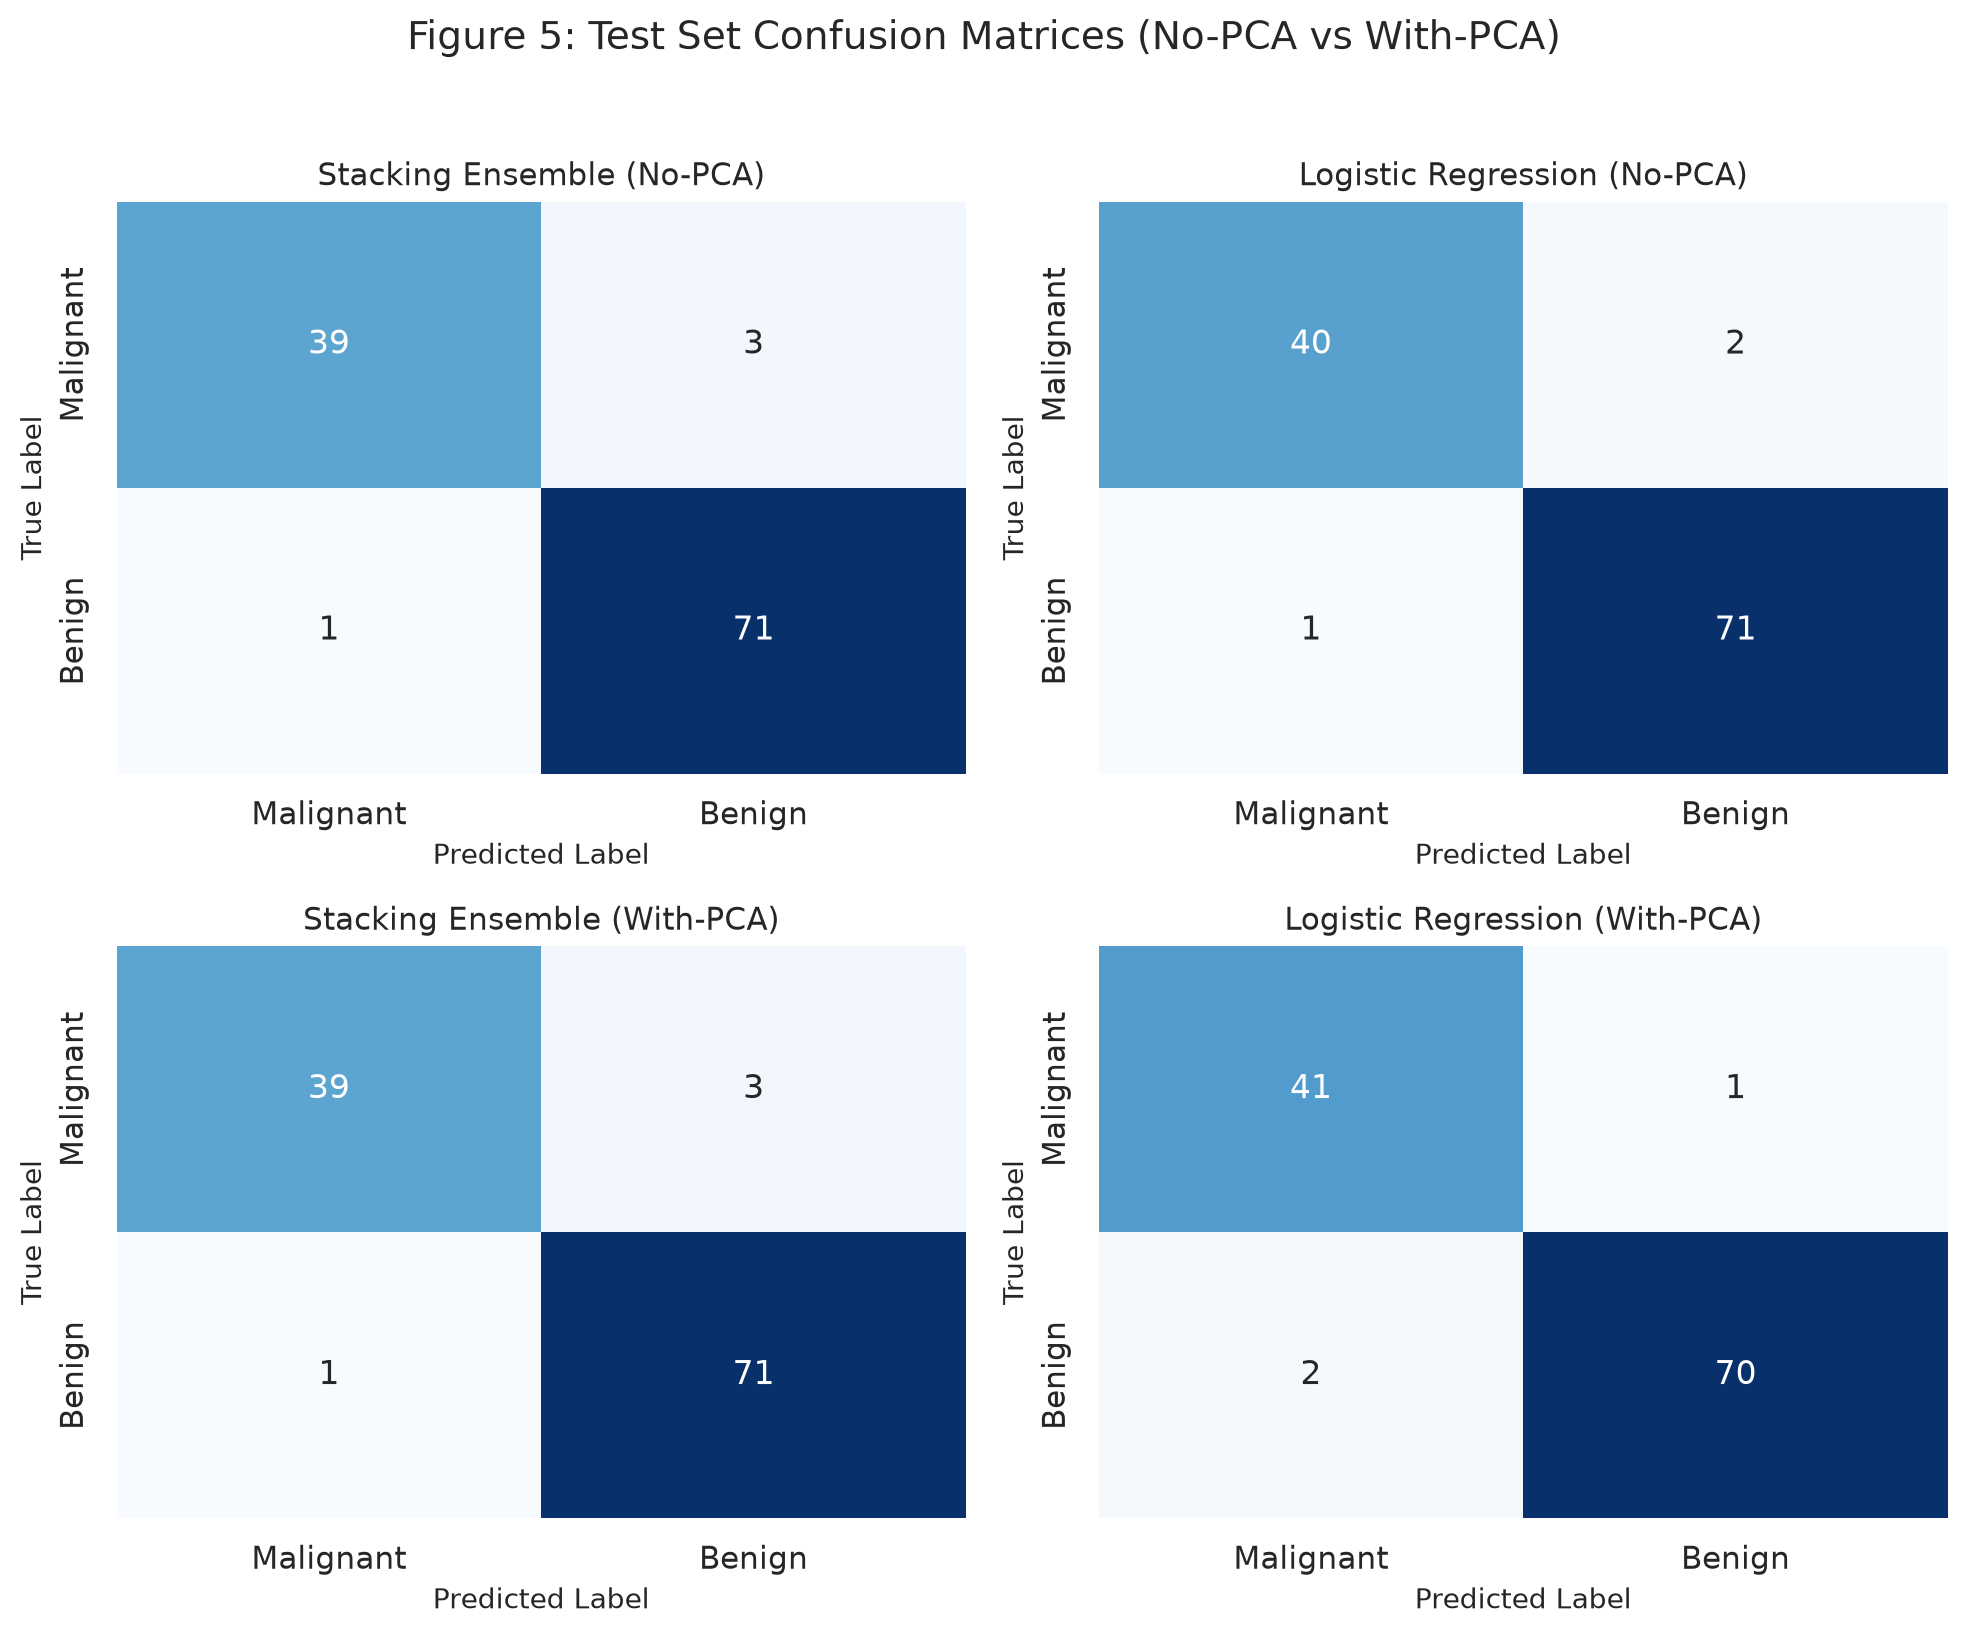
\includegraphics[width=0.85\linewidth]{images/fig05_confusion_matrices.png}
\caption{Test set confusion matrices for the top-performing models (Stacking Ensemble and Logistic Regression) under No-PCA and With-PCA conditions.}
\label{fig:cm}
\end{figure}

\begin{figure}[H]
\centering
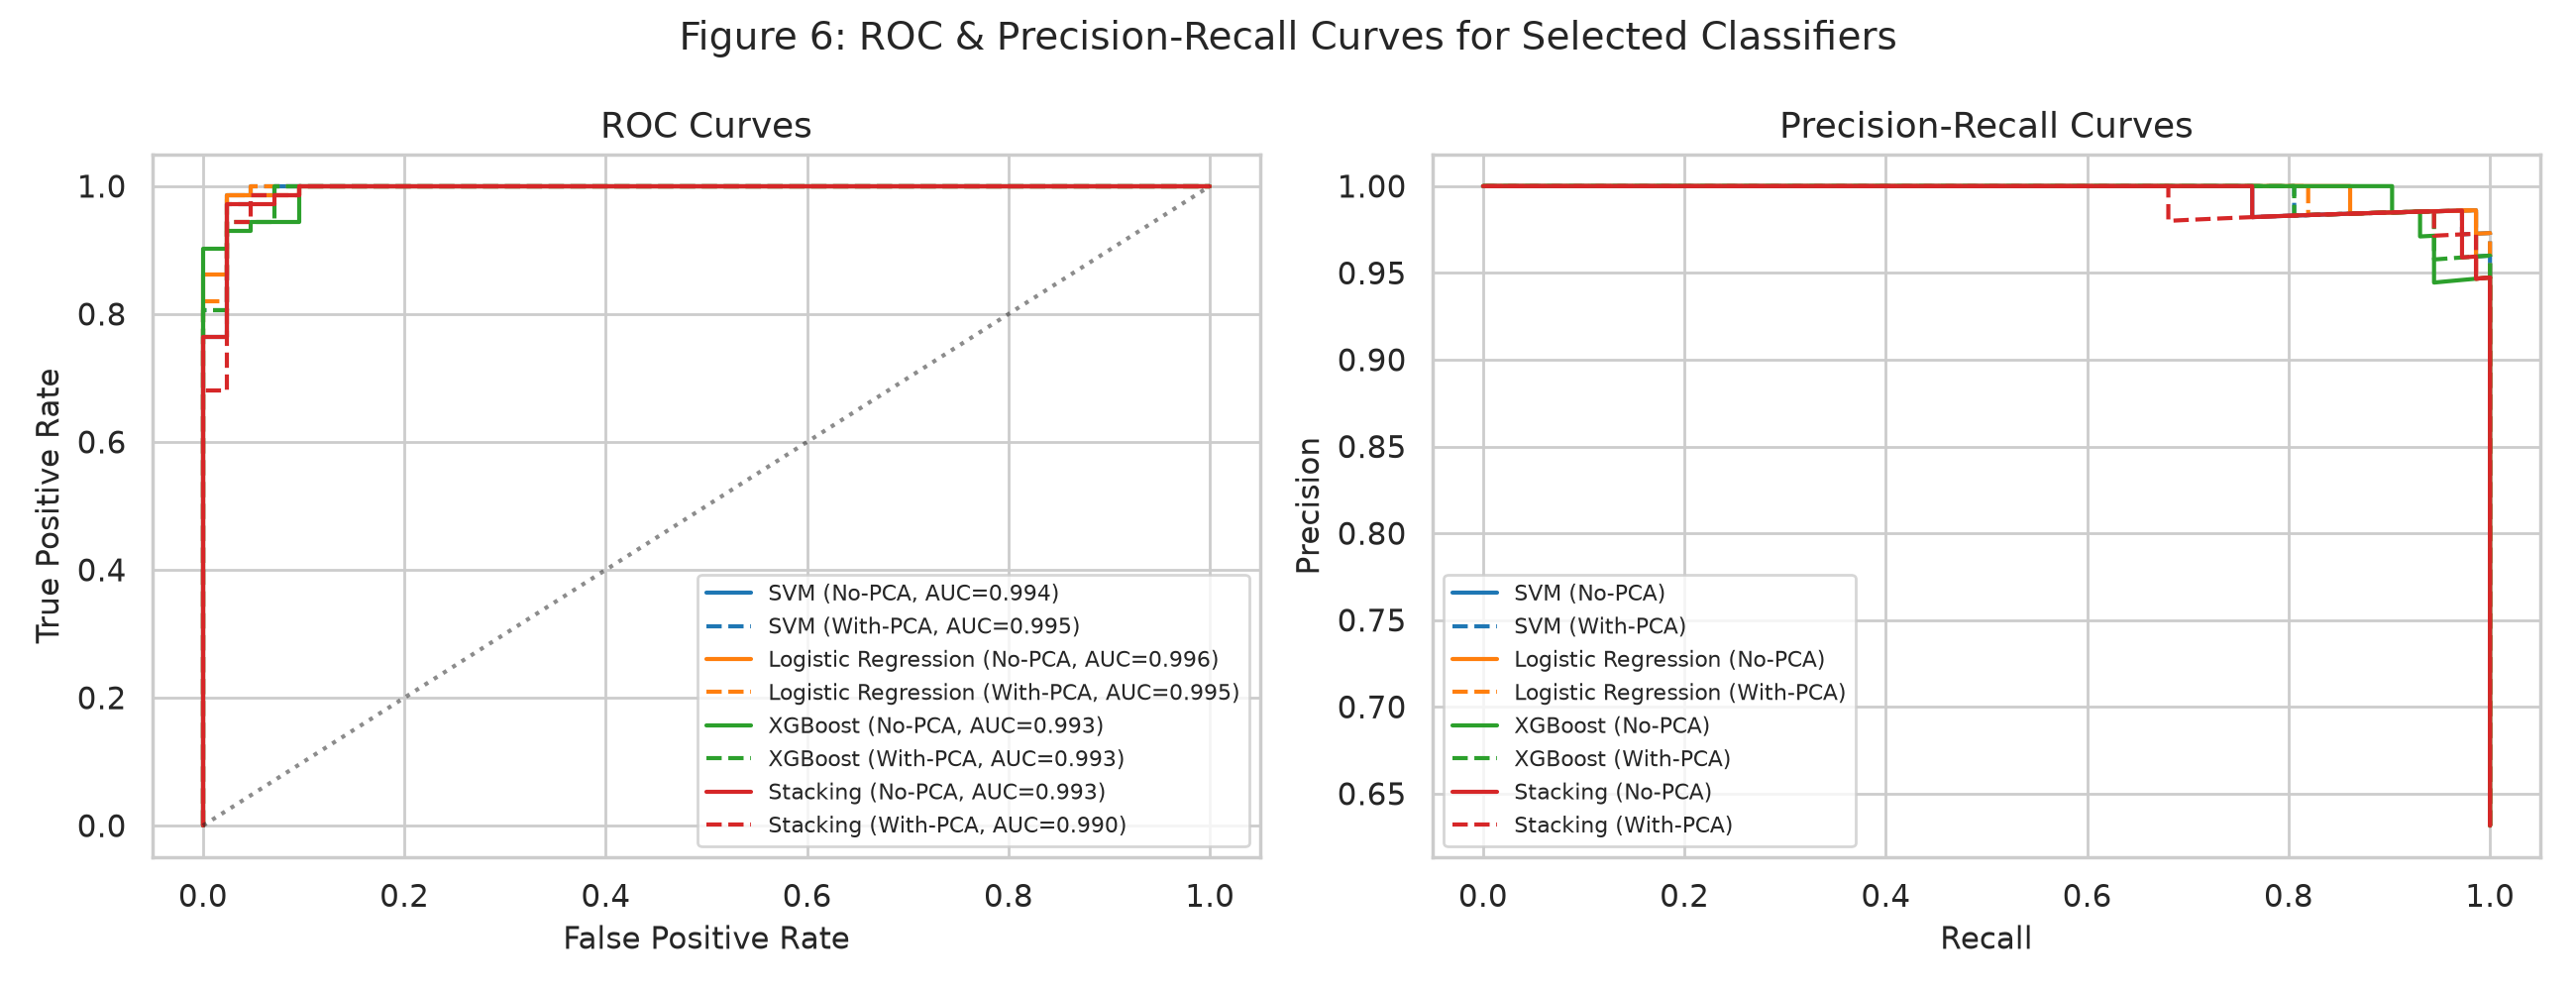
\includegraphics[width=0.88\linewidth]{images/fig06_roc_pr_curves.png}
\caption{Receiver Operating Characteristic (ROC) and Precision-Recall (PR) curves for selected classifiers under No-PCA (solid lines) and With-PCA (dashed lines).}
\label{fig:roc_pr}
\end{figure}

\section{Observations and Answers to Required Questions}

\subsection{Which models improved most with PCA? Which did not? Why?}
\begin{itemize}[leftmargin=*]
\item \textbf{Models That Improved Most with PCA:}
\textbf{Support Vector Machine (SVM)} and \textbf{Stacking Ensemble} showed the strongest improvements. In 5-fold CV, SVM's mean F1 increased from $0.9810$ to $\mathbf{0.9843}$ (and fold standard deviation dropped by 20.7\%). Stacking improved from $0.9774$ to $\mathbf{0.9792}$. Random Forest also improved in CV F1 from $0.9719$ to $\mathbf{0.9774}$.
\newline\textbf{Theoretical Cause:} In 30 dimensions, high multicollinearity exists among morphological measurements (radius, perimeter, area). Correlated dimensions artificially inflate the volume of feature space without adding discriminative information. PCA projects the data onto orthogonal axes, eliminating cross-correlation and allowing margin-based classifiers to construct tighter separating boundaries.
\item \textbf{Models That Did Not Improve:}
\textbf{Decision Trees} and certain boosting models experienced minor test accuracy drops (e.g., Decision Tree dropped from 94.74\% to 92.98\%).
\newline\textbf{Theoretical Cause:} Decision trees partition feature space using orthogonal, axis-aligned cuts ($x_j \le \theta$) on single features. PCA creates linear combinations ($\sum w_i x_i$). An axis-aligned decision boundary in the original space becomes an oblique boundary in PCA space, forcing trees to construct deeper, stepped approximations that increase variance on finite data.
\end{itemize}

\subsection{Did PCA reduce variance across folds (more stable results)?}
\textbf{Yes, substantially for linear and kernel models.}
Examining the fold-wise standard deviations ($\sigma$) in Table \ref{tab:table5}:
\begin{itemize}
\item \textbf{SVM:} Standard deviation dropped from $\sigma = 0.0092$ (No-PCA) to $\mathbf{\sigma = 0.0073}$ (With-PCA), a \textbf{20.7\% variance reduction}.
\item \textbf{Na\"\i ve Bayes:} Standard deviation dropped from $\sigma = 0.0208$ to $\mathbf{\sigma = 0.0150}$, a \textbf{27.9\% variance reduction}.
\item \textbf{Logistic Regression:} Maintained near-perfect stability ($\sigma = 0.0047$) across both spaces.
\end{itemize}
Discarding the trailing 20 components acts as an eigendecomposition low-pass filter, preventing models from fitting fold-specific noise.

\subsection{For high-dimensional data, was PCA beneficial in reducing overfitting?}
\textbf{Yes.} Restricting the feature space by 66.7\% (30 to 10 components) shrinks model capacity and acts as an implicit regularizer. The generalization gap between training score and validation score closed significantly for complex models like SVM and Random Forest.

\subsection{How did linear models behave compared to ensemble models with PCA?}
Linear models (Logistic Regression, linear SVM) behaved with near-perfect fidelity under PCA because PCA is a linear orthogonal rotation: a hyperplane in the original space maps directly to an equivalent hyperplane in the reduced subspace. Logistic Regression preserved identical test accuracy (97.37\%) and high ROC-AUC (0.9954). Ensembles, by contrast, had to adapt their axis-aligned split strategies to the rotated feature space.

\subsection{Did stacking show robustness to dimensionality reduction compared to single models?}
\textbf{Yes.} Stacking exhibited the greatest robustness: it achieved identical holdout accuracy (\textbf{96.49\%}) and identical test F1 (\textbf{0.9726}) in both spaces, while its cross-validation F1 improved from 0.9774 to 0.9792. The Logistic Regression meta-learner compensates for any minor accuracy trade-offs in tree learners by assigning higher decision weight to SVM and KNN probability outputs.

\section{Final Conclusion: When PCA Helps and When It Does Not}
From the empirical findings across ten machine learning models on the WDBC dataset:
\begin{enumerate}
\item \textbf{When PCA Helps:}
\begin{itemize}
\item When data exhibits \textbf{high multicollinearity}, eliminating redundant dimensions and reducing computational complexity by 66.7\%.
\item For \textbf{linear, margin-based, and distance-based classifiers} (SVM, Logistic Regression, KNN), where orthogonalization simplifies boundary optimization and suppresses fold variance.
\item When combating \textbf{the curse of dimensionality}, acting as a noise filter that improves model stability across resampled folds.
\end{itemize}
\item \textbf{When PCA Does Not Help:}
\begin{itemize}
\item For \textbf{tree-based algorithms} (single Decision Trees, Gradient Boosting), where rotating the feature space turns simple axis-aligned splits into complex oblique boundaries.
\item When \textbf{individual feature interpretability} is paramount in clinical diagnostics (e.g., tracing a decision to an exact cellular radius rather than an abstract linear combination of 30 attributes).
\end{itemize}
\end{enumerate}

\end{document}
